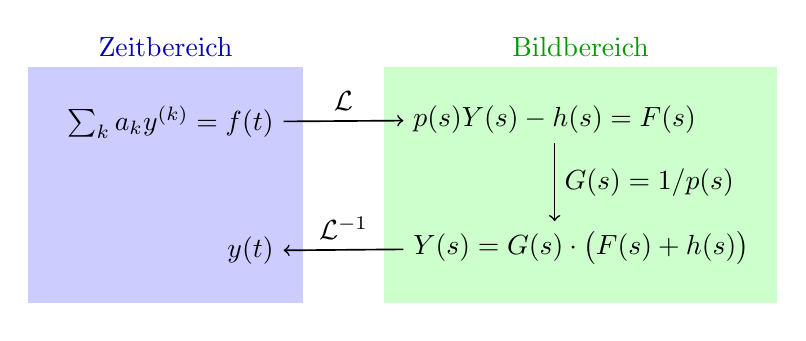
\begin{tikzpicture}[semithick]
  \node[fill=blue!20,
        minimum height=3cm,
        minimum width=3.5cm,
        anchor=east] (time) at (-.5, 0) {};

  \node[fill=green!20,
        minimum height=3cm,
        minimum width=5cm,
        anchor=west] (image) at (.5, 0) {};

  \node[minimum height=3.25cm,
        minimum width=1.5cm] (R) {};

  \node[above, color=blue!70!black] at (time.north)
    {Zeitbereich};

  \node[above, color=green!60!black] at (image.north)
    {Bildbereich};

  \node[anchor=north east, yshift=-5mm] (time-dgl) at (R.north west)
    {\(\sum_k a_k y^{(k)} = f(t)\)};

  \node[anchor=north west, yshift=-5mm] (image-dgl) at (R.north east)
    {\(p(s) Y(s) - h(s) = F(s) \)};

  \node[anchor=south west, yshift=5mm] (image-sol) at (R.south east)
    {\(Y(s) = G(s) \cdot \big( F(s) + h(s) \big)\)};

  \node[anchor=south east, yshift=5mm] (time-sol) at (R.south west)
    {\(y(t)\)};

  \draw[->] (time-dgl) to
    node[midway, above] {\(\mathcal{L}\)} (image-dgl);

  \draw[->] (image-dgl) to
    node[midway, right] {\(G(s) = 1/p(s)\)} (image-dgl |- image-sol.north);

  \draw[->] (image-sol) to
    node[midway, above] {\(\mathcal{L}^{-1}\)} (time-sol);

\end{tikzpicture}
